% !Mode:: "TeX:UTF-8"
%%% Local Variables:
%%% mode: latex
%%% TeX-master: t
%%% End:

\chapter{影像分类相关理论基础}
\label{cha:chap02}
%目标地物的识别分类一直是遥感影像解译中的重大任务。遥感影像分类任务依据是否使用地物类别先验知识分为监督分类和非监督分类。由于遥感影像多以非结构化、不精确的形式存在,缺乏完善的标记类别的规整数据。传统影像分割识别方法多以无监督的聚类分割辅以人工后处理的方法来完成遥感影像的解译工作。遥感影像数据固有的不确定性(“混合像元”、“同物异谱”和“同谱异物”等)使得模糊C-均值聚类方法成为遥感影像无监督聚类分割的优选方法,被广泛应用到遥感影像聚类分割识别任务中\cite{he2016remote}。另一方面,深度神经网络因其在特征提取方面效果显著,能够较好提取遥感影像复杂数据结构的隐含特征信息。并且,基于生成对抗网络模型的神经网络模型能够解决遥感影像分割中样本数不足的问题,因此具有重要的研究意义。

本课题主要从表征影像不确定性和小样本影像数据分类两个方面来研究遥感影像的分类识别方法。第~\ref{cha:chap03} 章研究内容是对当前的模糊聚类遥感影像无监督分割方法改进,能够更好地表达遥感影像“同物异谱”的不确定性;这部分工作基于遥感影像的模糊聚类分割基础知识;第~\ref{cha:chap04} 章则是结合深度神经网络相关方法,针对少标签样本的影像数据,提出基于生成对抗网络框架的遥感影像分割方法,该章节中的大量工作将基于深度学习中的卷积神经网络和图像语义分割相关的知识。所以本章将依次介绍遥感影像模糊聚类无监督分割方法,神经网络基础知识以及深度神经网络用于影像分割的网络设计方法和思想。

\section{遥感影像的模糊聚类分割基础}
\label{sec:chap02-1}
本课题中处理的遥感影像数据均为高分辨率遥感影像数据,文中主要研究面向对象的遥感影像模糊聚类方法。面向对象的模糊聚类方法主要包含影像分割,模糊聚类和后处理三个部分。后处理部分包含借助辅助软件人工处理相关的内容,不是本文研究重点。下面依次介绍影像分割和模糊聚类方法相关知识与算法原理。

\subsection{影像分割方法}
\label{subsec:chap02-1-1}
面向对象的影像分割是指对遥感影像分割划分,将邻域内同质性的像元当作一个整体,形成的影像分割单元区域内部的颜色、灰度、纹理等特性相似性较大,区域间的颜色、灰度、纹理等特性相异性较大。常见的影像分割根据分割类型可以划分为:边缘检测分割方法、阈值分割方法和基于区域的分割方法。边缘检测分割方法是通过Sobel、Canny、LOG 等滤波算子提取影像边缘,再将边缘连接起来形成边界,一般适用于灰度影像的分割。阈值分割方法通过比较像素与设定阈值大小关系,划分影像的前景和背景,该方法简单但不适用于较复杂的影像。基于区域的分割方法包含生长法和区域分裂合并法,其原理依据是影像中距离近的像素点相似性大,距离远的相似性小。基于区域的分割方法应用广泛,且分割效果较好。文中详细介绍两种常见的分割方法:Watershed 分水岭算法\cite{vincent1991watersheds} 和SLIC 超像素分割算法\cite{achanta2012slic}。

\subsubsection*{1. Watershed 分水岭算法}
\label{subsubsec:chap02-1-1-1}
Watershed 分水岭分割算法是一个非常经典的区域生长分割方法。算法的思想是把待分割图像想象成一个地理上的地形图,图像灰度值大小可看作地形高程值,图像每个局部极小值及其影响区域对应地形上的低洼处,即集水盆。两个集水盆汇合边界则为分水岭。分水岭算法如图~\ref{fig:watershed} 所示。

\begin{figure}[htb]
  \centering
  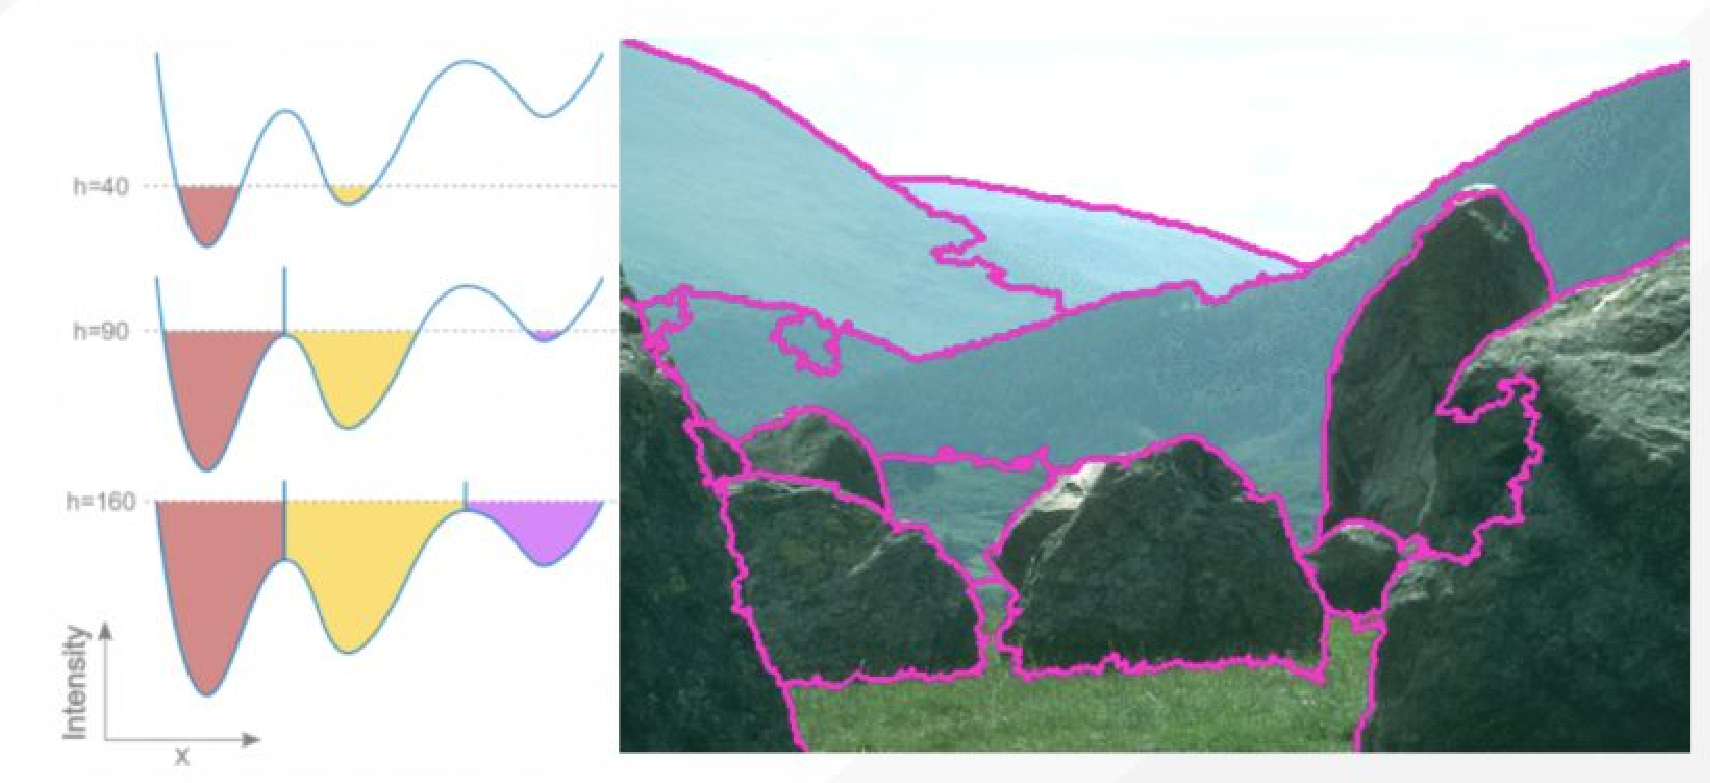
\includegraphics[width=0.7\textwidth]{figures/watershed}
  \caption{Watershed 分水岭算法示意图 }\label{fig:watershed}
\end{figure}

根据Watershed 分水岭算法原理,为得到图像的边缘信息,通常把梯度图像作为输入图像,即
\begin{equation}
  \label{eq:2-1}
  g(x,y) = \nabla f = \left[
    \begin{matrix}
      G_x \\
      G_y
    \end{matrix}
    \right] =
  \left[
    \begin{matrix}
      \frac{\partial f}{\partial x} \\
      \frac{\partial f}{\partial y}
    \end{matrix}
    \right]
\end{equation}
其中,$f(x,y)$表示原始图像,$g(x,y)$ 表示原始图像的梯度运算。假设$R_1,R_2,R_3,\cdots,R_m$ 表示待分割图像的极小区域的集合,$C(R_i)$ 表示为与极小区域$R_i$ 相关的流域,$n$ 表示溢流的增加数值(即在第$n$ 步时溢流的深度),$T[n]$ 表示满足梯度$g(x,y)<n$ 的所有像素点$(x,y)$ 的集合。对于一个给定流域,假设在第$n$ 步时极小区域$R_i$ 发生溢流,令$C_n(R_i)$ 为与极小区域$R_i$ 相关流域的一部分,即在溢流深度$n$ 时,在流域$C(R_i)$ 中形成的水平面构成的区域,$C_n(R_i)$ 为二值图像,可表示为:
\begin{equation}
  \label{eq:2-2}
  C_n(R_i) = C(R_i)\cup T[n]
\end{equation}
为防止分水岭算法产生的过度分割,通常设置阈值对梯度函数进行修改,以消除灰度的微小变化产生的过度分割。即
\begin{equation}
  \label{eq:2-3}
  g(x,y) = \max ( \nabla f(x,y),g_{\theta})
\end{equation}
式中,$g_{\theta}$ 表示阈值。

\subsubsection*{2. SLIC 超像素分割算法}
\label{subsubsec:chap02-1-1-1}
SLIC(Simple linear iterativeclustering),即简单的线性迭代聚类超像素分割方法。它采用$K$ 均值聚类方法高效地生成超像素,较以前的算法可以更好地获取分割边界,且有着更快的运行速度。

\begin{figure}[htb]
  \centering
  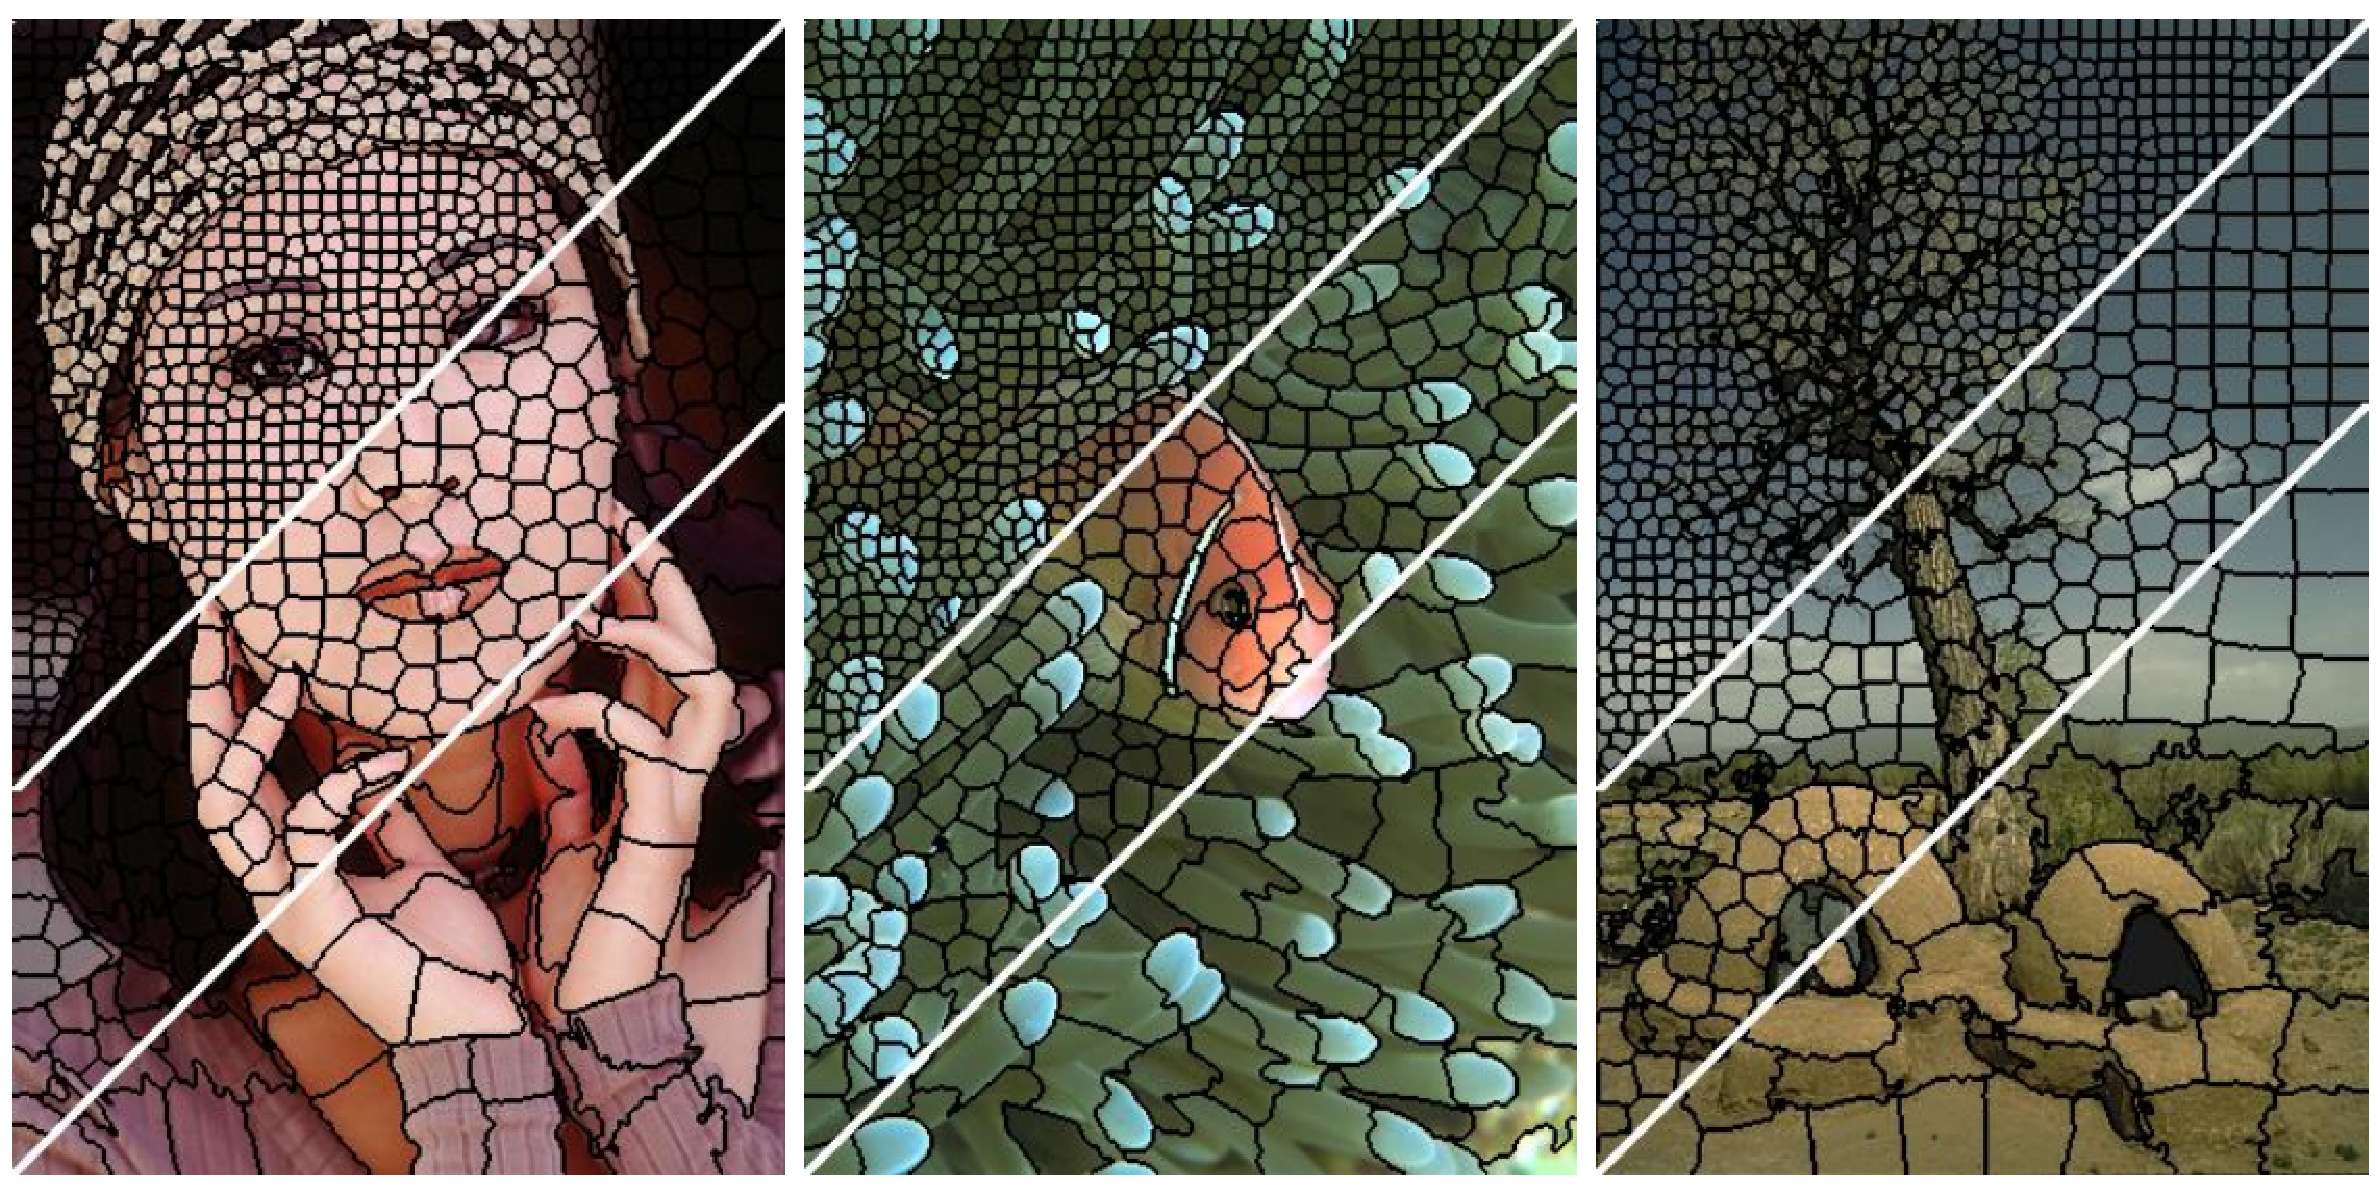
\includegraphics[width=0.8\textwidth]{figures/slic}
  \caption{SLIC 算法分割成尺寸为$64$,$256$ 和$1024$ 的超像素单元}\label{fig:slic}
\end{figure}

SLIC 算法将彩色图像转化为CIELAB颜色空间和XY坐标下的5维特征向量,即位于$(x,y)$ 处的像元在CIELAB颜色空间表示为$[l,a,b,x,y]$ ,CIELAB 空间由LAB 色彩模型表征,$l$ 为亮度,$a,b$ 为色彩值。对有$N$ 个像素点的图像,预分割为$K$ 个相同尺寸的超像素,则每个超像素单元的大小为$N/ K$, 则相邻种子间的步长为$S = \sqrt{N/K}$ 。SLIC 的搜索范围限制为$2S*2S$,对于每个搜索到的像素点,分别计算它和该种子点的距离,包括颜色距离和空间距离。距离计算方法如下
\begin{equation}
  \label{eq:2-5}
  \begin{split}
    d_c &= \sqrt{(l_j-l_i)^2 + (a_j-a_i)^2 + (b_j - b_i)^2} \\
    d_s &= \sqrt{(x_j-x_i)^2 + (y_j-y_i)^2} \\
    D &= \sqrt{(\frac{d_c}{N_c})^2 + (\frac{d_s}{N_s})^2}
  \end{split}
\end{equation}
式中,$d_c$ 表示颜色距离,$d_s$ 表示空间距离, $N_s$ 表示类内最大空间距离,定义为
\begin{equation}
  \label{eq:2-6}
  N_s = S = \sqrt{N/K}
\end{equation}
$N_c$ 为最大的颜色距离,取值随具体的图片而定,实验中一般取一个固定常数$m$ (取值范围为$(1\leq m \leq 40)$,一般取$10$。$D$ 表示总距离,即最终的距离度量为:
\begin{equation}
  \label{eq:2-7}
  D = \sqrt{(\frac{d_c}{m})^2 + (\frac{d_s}{S})^2}
\end{equation}
通过迭代优化直至误差收敛即可完成图像的超像素分割。图~\ref{fig:slic} 所示为基于SLIC 算法分别将图像大约分成$64$,$256$ 和$1024$ 三个尺寸的结果。



\subsection{模糊聚类方法}
\label{subsec:chap02-1-2}

模糊C 均值(fuzzy c-means, FCM)聚类方法是结合模糊数学不确定性理论对K-means 聚类方法的改进。与K-means 算法中依据欧式距离作为类别划分依据的硬分类不同,FCM 算法是以隶属度为类别划分依据的软分类方法。FCM 方法是一种柔性的模糊划分,因此FCM 比K-means 算法更能突出遥感影像不确定性的特点。在复杂、高维遥感影像实际应用中,FCM 算法效果显著优于K-means 算法。

介绍FCM 方法前,先引入模糊集合中隶属度函数的概念。隶属度函数表示一个对象$x$ 属于集合$A$ 的程度的函数,记作$\mu_{A}(x)$ 。其自变量是可能属于集合$A$ 的所有元素,因变量是$[0,1]$ 区间内的值,即满足$0 \leq \mu_{A}(x) \leq 1$ 。$\mu_{A}(x) = 0$ 表示元素$x$ 不属于集合$A$,等价于普通集合中$x \notin A$;$\mu_{A}(x) = 1$ 则表示$x$ 完全隶属于$A$,等价于$x \in A$。一个定义在论域$X$ 上的隶属度函数就定义了一个模糊集,即模糊集$A$ 可由其成员$x$ 的隶属函数$\mu (x)$ 来刻画,如式~\ref{eq:2-8}:
\begin{equation}
  \label{eq:2-8}
  A = \{(x,\mu (x)) | \forall x \in X,\mu (x) \in [0,1] \}
\end{equation}

有了模糊集合与隶属度的概念,一个元素属于模糊集合就不是硬性的了。对应到聚类问题中,可以把聚类生成的簇看作模糊集合,因此,每个样本点隶属于簇的隶属度就是$[0,1]$ 区间内的值。

假定数据集$X=\{x_1,x_2,\cdots,x_n \}$,把数据划分为$m$ 个类别,聚类中心为$C = \{c_1,c_2,\cdots,c_m \}$,样本$x_i$ 属于类别$c_j$ 的隶属度为$\mu_{ji}$,则FCM 方法优化的目标函数为式~\ref{eq:2-9}:
\begin{equation}
  \label{eq:2-9}
  J= \sum_{j=1}^m \sum_{i=1}^n \mu_{ji}^k||x_i-c_j||^2
\end{equation}
其中$1 \leq k \leq \infty$ 为模糊指数,目标函数$J$ 的约束条件为式~\ref{eq:2-10}:
\begin{equation}
  \label{eq:2-10}
  \sum_{j=1}^m \mu_{ij} = 1, i=1,2,\cdots,n
\end{equation}
通过拉格朗日乘子法将约束条件写入目标函数式中,则:
\begin{equation}
  \label{eq:2-11}
  J = \sum_{j=1}^m \sum_{i=1}^n \mu_{ji}^k||x_i-c_j||^2 + \lambda_1(\sum_{j=1}^m \mu_{j1} -1 )  + \cdots + \lambda_i(\sum_{j=1}^m \mu_{ji} -1 ) + \cdots + \lambda_n(\sum_{j=1}^m \mu_{jn} -1 )
\end{equation}

令式~\ref{eq:2-11} 分别对$\mu_{ji}$ 和$c_j$ 求偏导并让求导结果等于$0$,化简求解,有:
\begin{equation}
  \label{eq:2-12}
  \mu_{ji} = \frac{1}{\sum_{s=1}^m(\frac{||x_i-c_j||}{||x_i-c_s||})^{(\frac{2}{k-1})}}
\end{equation}
和
\begin{equation}
  \label{eq:2-13}
  c_j = \frac{\sum_{i=1}^n(x_i\mu_{ji}^k)}{\sum_{i=1}^n\mu_{ji}^k} = \sum_{i=1}^n \frac{\mu_{ji}^k}{\sum_{i=1}^n\mu_{ji}^k}x_i
\end{equation}

依据式~\ref{eq:2-12} 和~\ref{eq:2-13} 中的求导结果对FCM 方法聚类中心迭代优化,直到误差小于阈值或到达最大迭代次数,迭代停止。

迭代停止时,样本$x_i$ 对所有聚类中心$[c_1,c_2,\cdots,c_j,\cdots,c_m]$ 的隶属度矩阵向量为$U_{\cdot i} = [\mu_{1i},\mu_{2i},\cdots,\mu_{ji},\cdots,\mu_{mi}]$,样本$x_i$ 最终归属的类别依据隶属度最大化原则划分为类别$c_K$,则有:
\begin{equation}
  \label{eq:2-14}
  K = \mathop{\arg\max}_{j} U_{\cdot i} = \mathop{\arg\max}_{j} (\mu_{1i},\mu_{2i},\cdots,\mu_{ji},\cdots,\mu_{mi})
\end{equation}
依据式~\ref{eq:2-14} 对每个样本找到其隶属度最大的类别,即可完成整个数据集的模糊聚类划分。

\section{基于神经网络的影像分割相关理论}
\label{sec:chap02-2}
深度学习是以人工神经网络为架构,通过多隐层网络结构提取高层抽象特征,对数据进行表征学习的算法。常见的深度学习框架包含深度神经网络(Deep neural network, DNN)、深度置信网络(Deep belief network, DBN)、递归神经网络(Recurrent neural network, RNN)和卷积神经网络(Convolutional neural network, CNN)等\cite{krizhevsky2012imagenet} 。 与其他网络结构相比,CNN 利用输入数据的二维结构信息,在图像分类与识别、图像语义分割等视觉任务中能够给出更好的结果。


\subsection{卷积神经网络基础}
\label{subsec:chap02-2-1}
CNN 是一种具有卷积结构的深度前馈神经网络,使用反向传播(Backpropagation,BP)算法进行训练,主要用来处理图像信息。CNN 网络结构一般由卷积层(Convolutional layer)、池化层(Pooling layer)和全连接层(Full connected layer)交叉堆叠而成。卷积层和池化层用于提取图像高阶特征,具有局部连接、权值共享、下采样等特性。全连接层起到图像“分类器”的作用,将学到的“分布式特征表示”映射到样本标记空间。

\subsubsection*{1. 卷积层}
\label{subsec:chap02-2-1-1}
卷积(Convolution)是分析数学中的一种运算,被广泛应用到信号处理与图像处理中。因为图像是两维结构数据,图像处理中常用二维卷积运算。给定一个图像$X \in \mathbb{R}^{M \times N}$,和滤波器$W \in \mathbb{R}^{m \times n}$, 一般满足$m \ll M, n \ll N$,其卷积输出:
\begin{equation}
  \label{eq:2-15}
  Y = X \otimes W
\end{equation}
式中,$\otimes$ 是卷积运算。 输出特征图上某点$(i,j)$ 的值可由式\ref{eq:2-16}计算得到:
\begin{equation}
  \label{eq:2-16}
  y_{ij} = \sum_{u=1}^m\sum_{v=1}^n w_{uv}\cdot x_{i-u+1,j-v+1} 
\end{equation}

CNN 最核心结构是卷积层,每个卷积层均包含一个或多个二维平面,该二维平面称作CNN 网络的特征图(Feature map)。同一特征图内神经元共享权重和偏置项,且每一个神经元与上一层的区域局部连接。CNN 中共享的权重称为卷积核(Convolutional kernel),利用卷积核对上一层的特征图进行卷积运算可以提取影像特征产生下一层网络的输出层。如图~\ref{fig:conv_op} 所示,图中使用大小为$3\times3$的卷积核,输入图像大小为$5\times5$,卷积核从左上方以$1$ 个像素点的步长(Stripe)开始滑动,图像中像素点与卷积核之间卷积运算后的输出到特征图上的对应位置。

\begin{figure}[htbp]
  \centering
  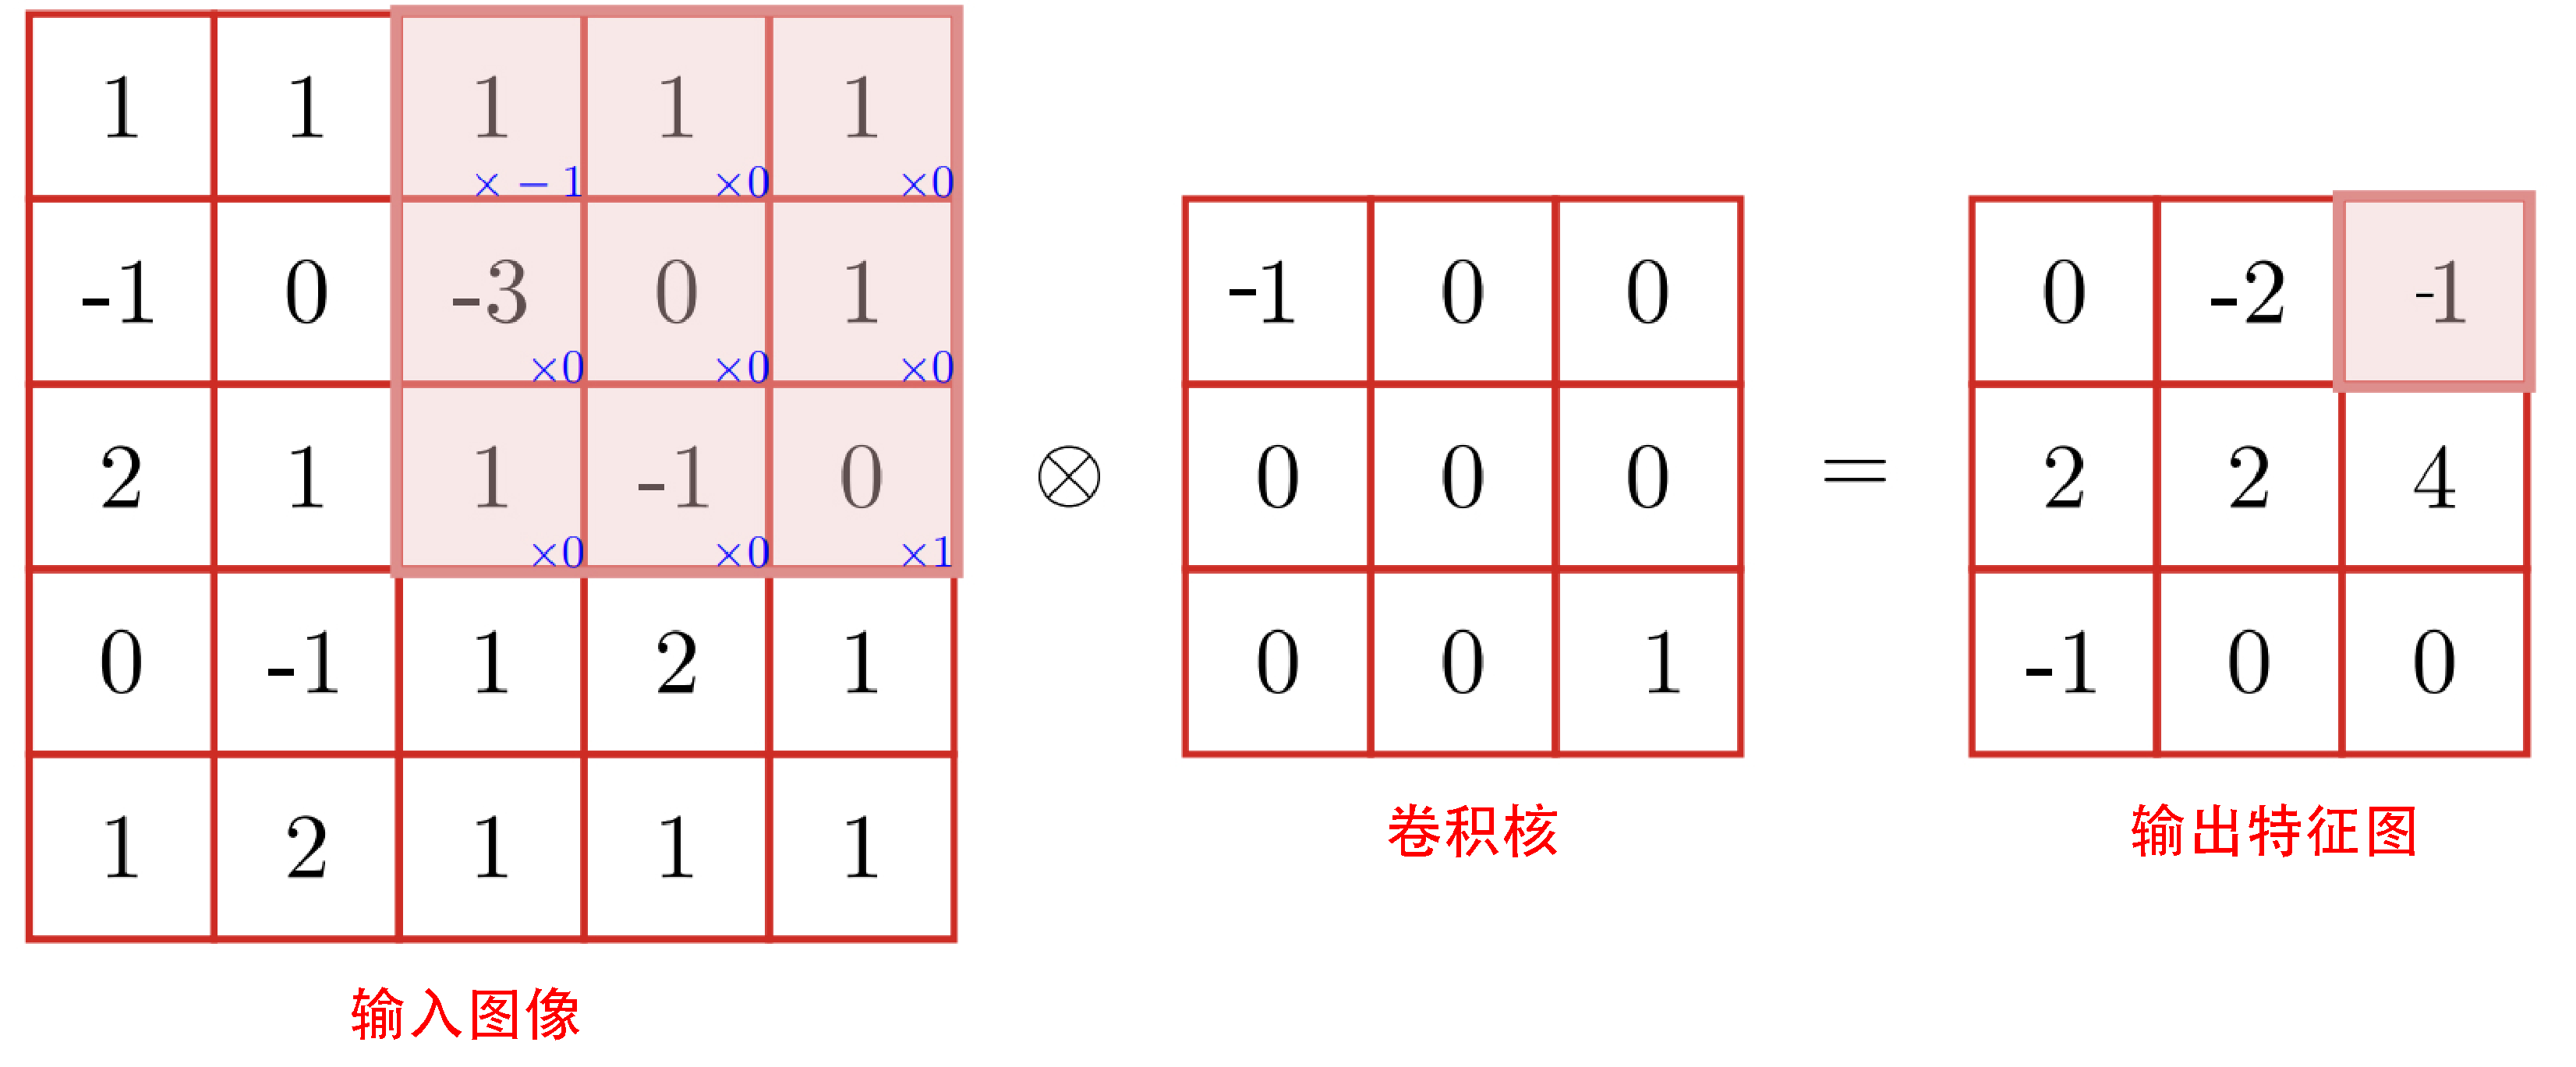
\includegraphics[width=0.8\textwidth]{figures/conv_op}
  \caption{图像卷积示意图}\label{fig:conv_op}
\end{figure}

图像卷积运算时,与全连接模式中每个像素点对应一个独立的计算权值不同,所有位置的输出神经元均使用一个卷积核计算权值,这样做的好处是既减少参数的数量,又利用了图像特征的局部性特点。图像卷积中,每个卷积核都可以提取图像的一种特征,所以一般设置多个卷积核,利用不同的卷积核来提取图像不同的特征。

卷积计算中第$l$ 层的输入是第$l-1$ 层的卷积输出特征图,假定第$l-1$ 层输入大小为$X_{l-1} \times X_{l-1}$,卷积核大小为$K \times K$,滑动步长为$S$,边界填充(Padding)大小为$P$,$l-1$ 层的输出特征图(即第$l$ 层的输入)的大小为$X_l \times X_l$,可由式\ref{eq:2-17} 计算得到:
\begin{equation}
  \label{eq:2-17}
  X_l = \lfloor \frac{X_{l-1} - K + 2 \times P}{S} \rfloor + 1
\end{equation}

卷积操作是线性的,线性模型的特点为任意线性模型的组合仍然是线性模型。线性神经网络无法解决实际复杂的非线性问题。为每个卷积输出添加一个非线性函数,神经网络模型就不再是线性的,这个非线性函数就是激活函数。常用的激活函数有Sigmoid、TanHyperbolic(tanh) 和线性整流函数(Rectified linear unit, ReLU) 函数等。当前卷积网络常用的是ReLU 激活函数,ReLU 函数的表达式如下:
\begin{equation}
  \label{eq:2-17-1}
  f(x) = \max(x,0)
\end{equation}
相比Sigmoid 和tanh 函数,ReLU 对于梯度训练的收敛有巨大加速作用,反向传播训练时不易饱和,另外ReLU 函数简单,运算量很小,因此广泛使用到卷积网络非线性激活中。

\subsubsection*{2. 池化层}
\label{subsec:chap02-2-1-2}
池化层又叫下采样层(Subsampling layer),能够缩小特征图尺寸,其作用是进行特征选择,降低特征数量,使特征更加抽象。卷积层虽然可以显著减少网络中连接参数的数量,但特征映射组中的神经元个数并没有显著减少。在卷积层后面加上一个池化层,可以降低下一层待处理的数据量,实现特征降维,一定程度上防止过拟合。

假定池化层的输入特征图为$X \in \mathbb{R}^{M \times N}$ ,将其划分为很多区域$R_{m,n},1 \leq m \leq M, 1 \leq n \leq N$,这些区域可以重叠,也可以不重叠。池化层通过池化函数对特征图的每个区域$R_{m,n}$ 进行下采样,得到一个值作为这个区域的概括。根据采样的方式不同,常用的池化函数有以下两种:
\begin{enumerate}[1. ]
\label{list:1}
\item 最大池化(Maximum pooling)
最大池化是选取区域内所有神经元的最大值作为池化输出。
\begin{equation}
  \label{eq:2-18}
  Y_{m,n} = \mathop{\max}_{i \in R_{m,n}} x_i
\end{equation}
其中,$x_i$ 为区域$R_k$ 内每个神经元的激活值。

\item 平均池化(Average pooling)
平均池化是选取区域内所有神经元激活值的和的平均值。
\begin{equation}
  \label{eq:2-19}
  Y_{m,n} =  \frac{1}{|R_{m,n}|}\mathbb{\sum}_{i \in R_{m,n}} x_i
\end{equation}
\end{enumerate}
对输入特征图的所有区域进行下采样,就可以得到池化层的输出特征图$Y = \{ Y_{m,n}\},1 \leq m \leq M, 1 \leq n \leq N$ 。

\begin{figure}[htbp]
  \centering
  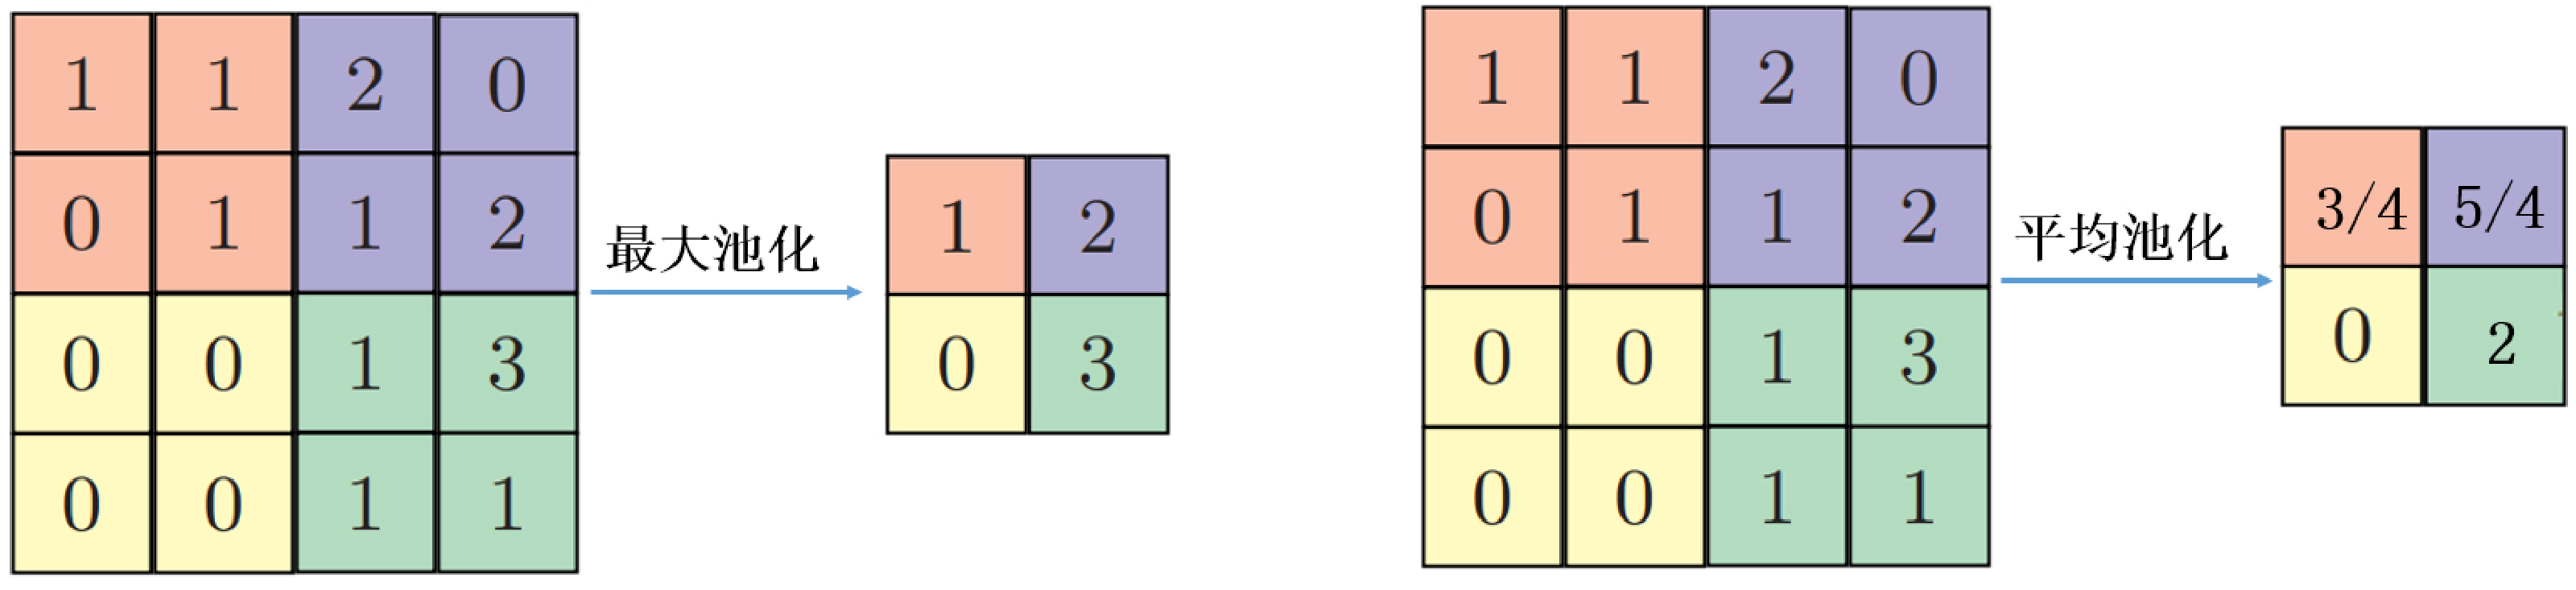
\includegraphics[width=0.9\textwidth]{figures/pooling}
  \caption{最大池化与平均池化}\label{fig:pooling}
\end{figure}

图如~\ref{fig:pooling} 所示,输入特征图大小为$4 \times 4$,池化函数核为$2 \times 2$,滑动步长为$2$ ,分别进行最大池化和平均池化操作,得到不同的池化输出特征图。

在卷积网络的最后,往往会接入一两层的全连接层。全连接层将卷积输出的二维特征“拍平”,转化成一个一维向量。全连接层对卷积输出特征高度提取,方便交给最后的分类器(如SVM 分类器、Softmax 分类器等)实现图像分类。

\subsubsection*{3. 典型的卷积网络结构}
\label{subsec:chap02-2-1-3}

一个典型的卷积网络由卷积层、池化层和全连接层交叉堆叠而成。如图~\ref{fig:cnn_structure} 所示,通常一个卷积块由连续的$M$ 个卷积层和$b$ 个池化层拼接而成($M$ 一般取$1\sim 4$,$b$ 可取$0$或$1$), 一个完整的用于分类任务的卷积网络结构通常由$N$ 个堆叠的卷积块后接$K$ 个全连接层组成($N$ 一般取$1\sim 100$,$K$ 取$1 \sim 2$)。CNN 中多层网络模型使得网络对不同形态的图像具有优秀的适应能力,它可以拟合高分影像中因地物尺度不一、拍摄角度不同等原因形成的复杂特征,从而有效提高分影像的分类识别精度。

\begin{figure}[htb]
  \centering
  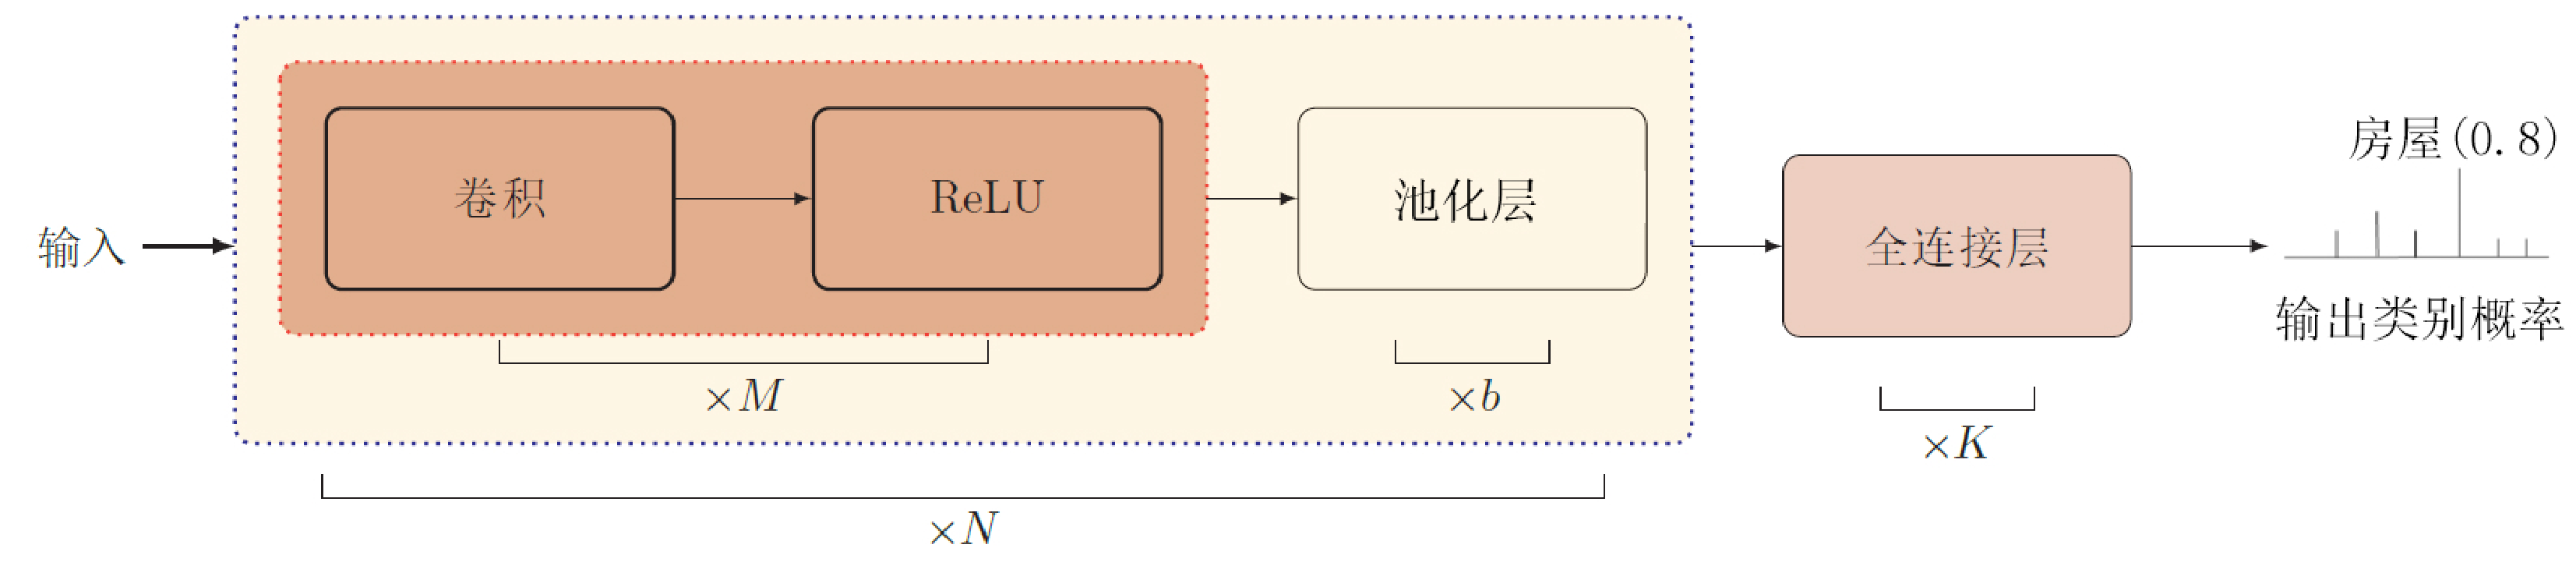
\includegraphics[width=1.0\textwidth]{figures/cnn_structure}
  \caption{典型的卷积网络结构}\label{fig:cnn_structure}
\end{figure}

\subsection{基于全卷积网络的图像分割}
\label{subsec:chap02-2-1}
传统的卷积神经网络最右端结构通常连接全连接层,它会将原来二维矩阵压缩成一维的,从而丢失图像的空间位置信息,且网络输出常为输入图像属于某一类别的概率。与分类对整张图片类别预测不同,图像的语义分割是对目标图像的每个像素点进行语义分类,即语义分割是从像素级对图像进行类别预测。全卷积神经网络(Fully convolutional network,FCN)\cite{long2015fully} 由Jonathan Long 等人于2016年提出,其创造性地利用卷积层替代分类网络中的全连接层,进而保证网络输出为二维分割图,使用反卷积(Deconvolution)的上采样策略,得到一个与原图尺寸大小相同的分割图,实现图像语义分割像素级的预测。图像语义分割应用到遥感领域即为遥感影像的分类。图~\ref{fig:fcn_structure} 为遥感影像分割的全卷积网络结构示意图,全卷积网络将学习到的遥感影像判别特征解码映射到高分辨率空间,完成影像的像素级分类。

\begin{figure}[htb]
  \centering
  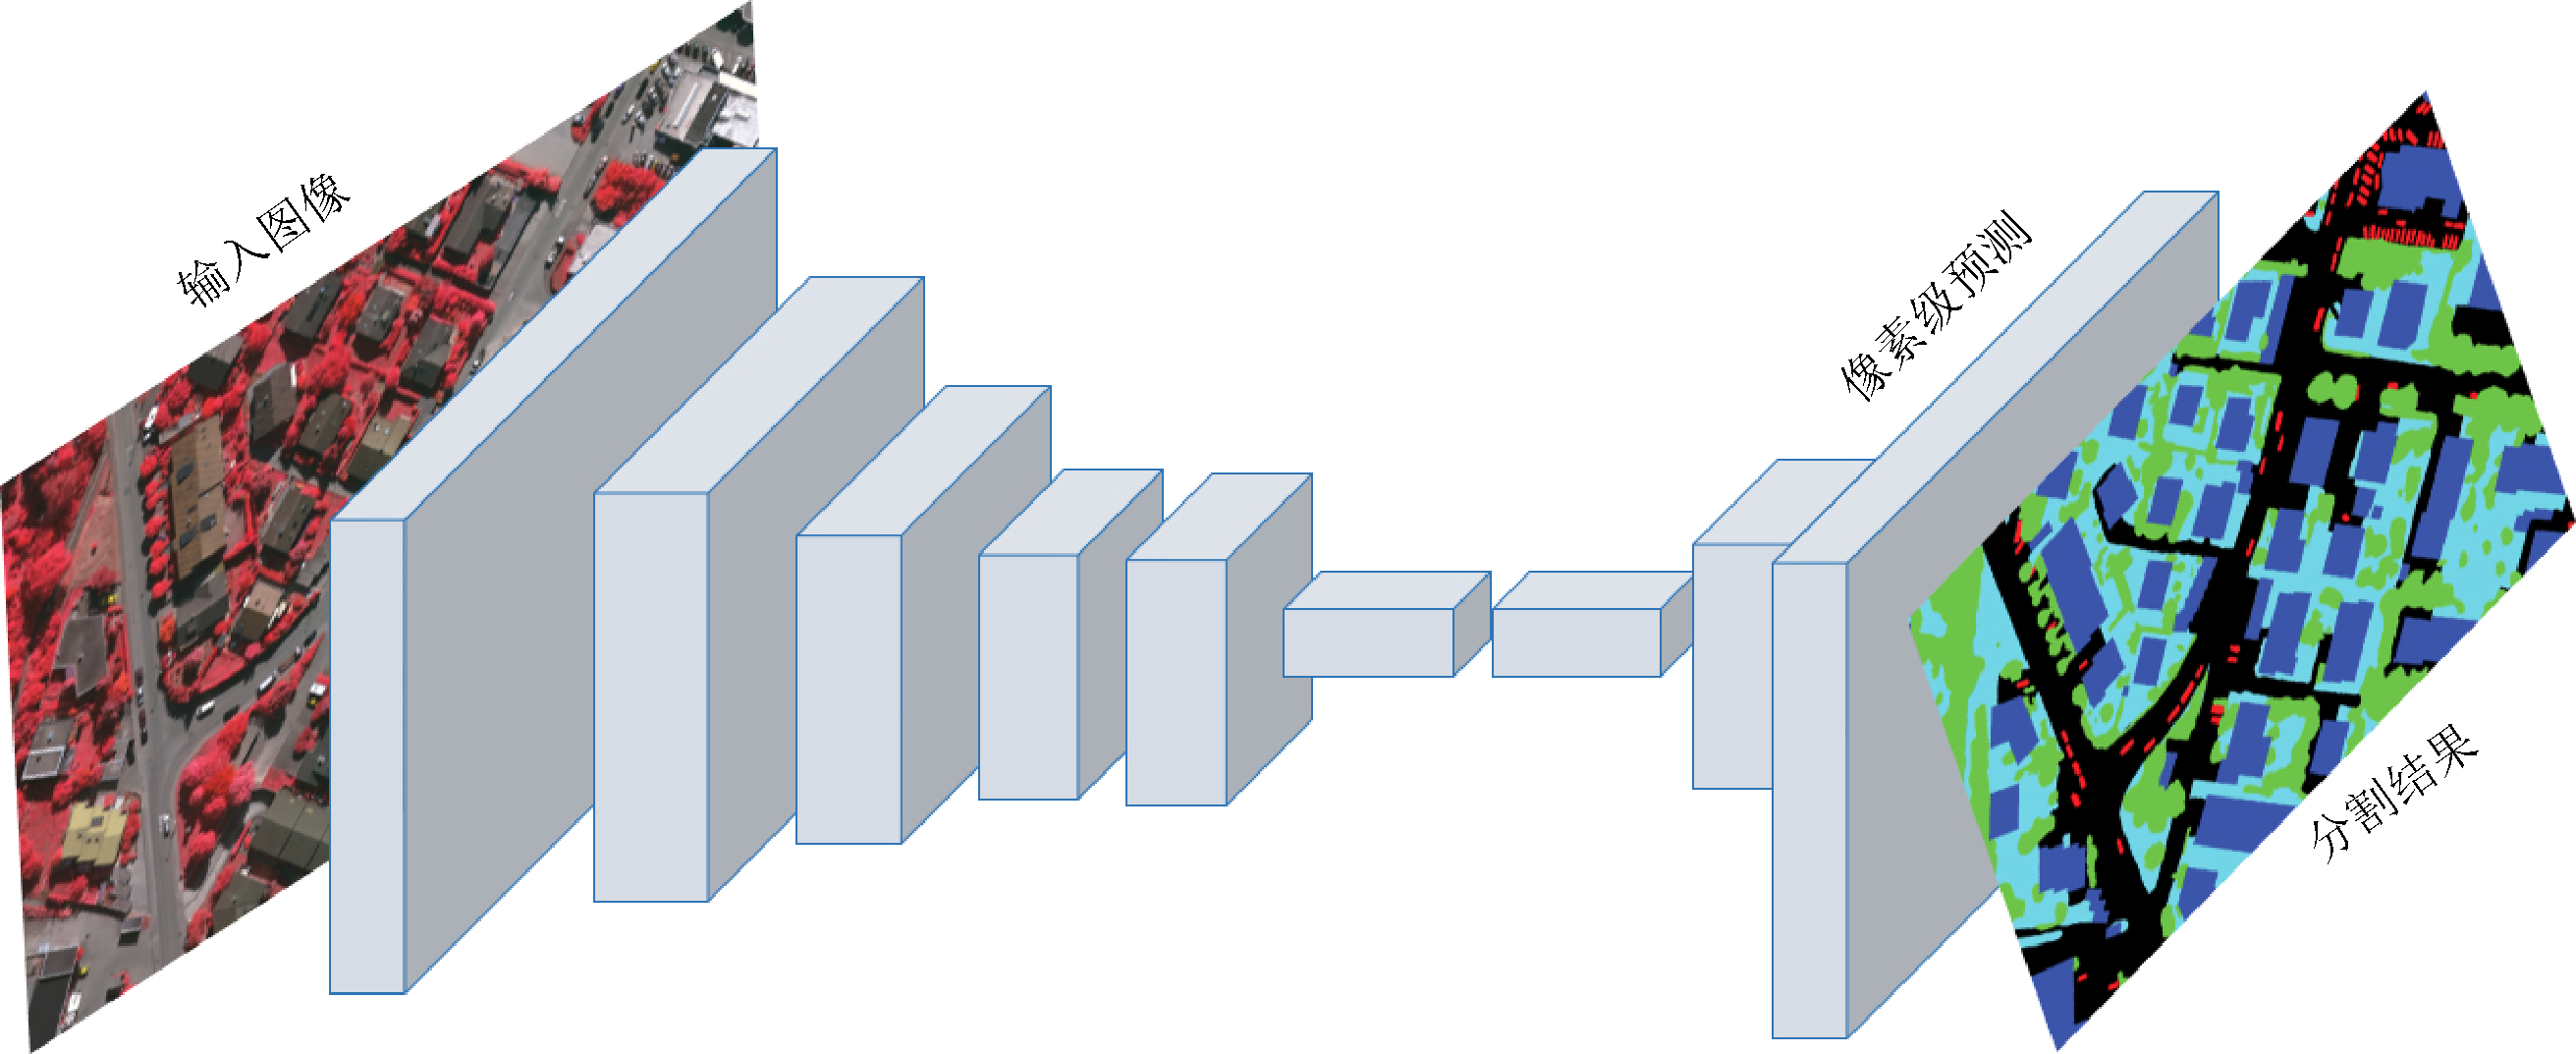
\includegraphics[width=0.9\textwidth]{figures/FCN}
  \caption{影像分割网络结构示意图}\label{fig:fcn_structure}
\end{figure}

\subsubsection*{1. 反卷积}
\label{subsec:chap02-2-2-1}
反卷积,又叫转置卷积,是一种上采样操作,可以理解为下采样的逆过程。卷积运算是一个下采样过程,一般通过卷积操作实现高维特征到低维特征的转换。如对输入$4\times 4$ 的二维特征,用大小$3\times 3$ 的核,做步长为$1$ 的卷积运算得到$2\times 2$ 的特征输出。反卷积则实现低维特征到高维特征的转换。与之对应,反卷积对输入为$2\times 2$ 的二维特征,使用$3\times 3$ 的核操作得到$4\times 4$ 的输出。如图~\ref{fig:deconv} 所示,输入特征大小$2\times 2$,核大小$3\times 3$,步长$s=1$,填充补0为$p=2$,经过反卷积处理输出尺寸上采样到$4\times 4$, 图中显示了反卷积上采样的计算过程。

\begin{figure}[htb]
  \centering
  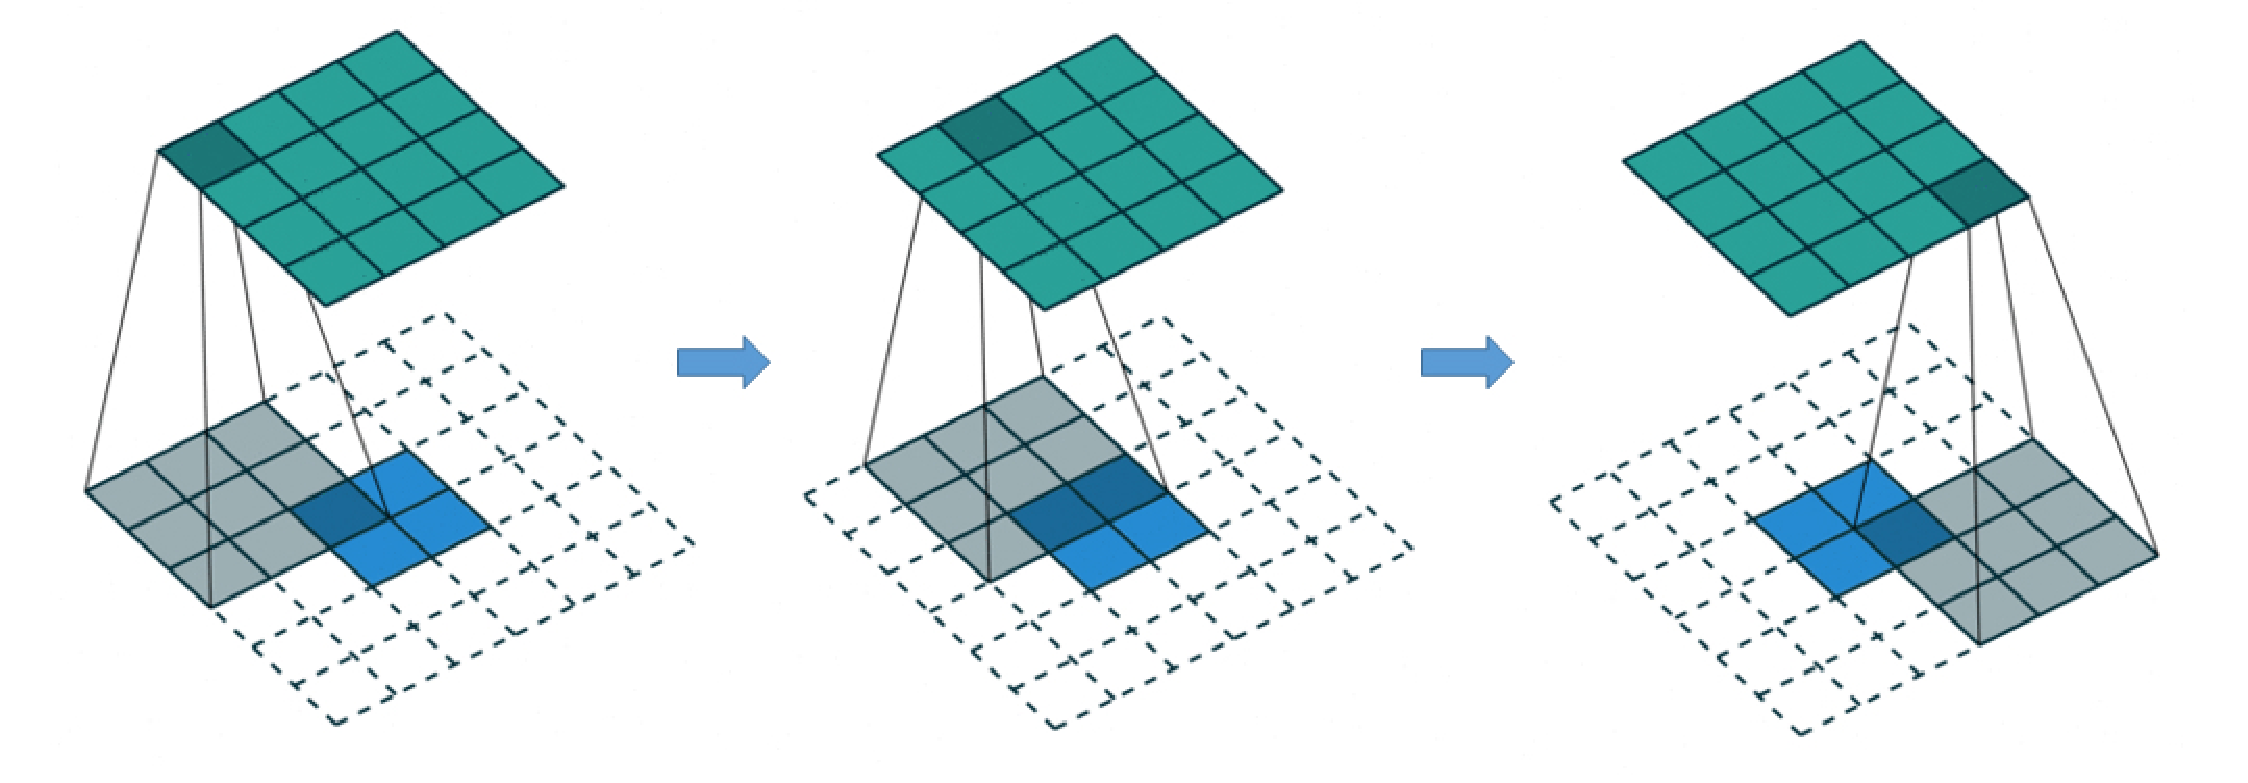
\includegraphics[width=0.8\textwidth]{figures/deconv}
  \caption{反卷积上采样过程}\label{fig:deconv}
\end{figure}

反卷积是卷积运算形式上转置的映射关系。对一个大小为$X\times X$的图像$\textit{I}$,和大小为$K\times K$ 的卷积核,进行步长为$S \geq 1$ 的反卷积运算,先对图像$\textit{I}$ 进行两端补零$P=K-1$,并且在每两个像素间填充$S-1$ 个$0$,最后进行步长为$1$ 的卷积操作,得到反卷积的输出结果,设输出特征维度为$O \times O$ ,满足:
\begin{equation}
  \label{eq:2-19}
  O = S \times (X - 1) + K
\end{equation}

\subsubsection*{2. FCN 网络图像分割}
\label{subsec:chap02-2-2-2}
FCN 网络由卷积特征提取和反卷积上采样两部分组成。FCN 特征提取阶段,为了加快网络训练速度,常使用在ImagaNet 等数据集上训练好的网络权值初始化FCN 网络参数,如对训练好的AlexNet\cite{krizhevsky2012imagenet} 或VGG\cite{simonyan2014very} 网络权值,选取除全连接层的权值参数初始化FCN 网络。输入图片经卷积池化层处理后特征图尺寸变小,所以特征图需要被上采样为输入图片相同尺寸。FCN 使用反卷积层做上采样将特征图尺寸调整为原输入图像大小。 同时,为了得到更精细的分割结果,FCN 中使用跳层连接(Skip connections)将下采样阶段和上采样阶段相同尺寸的特征图融合。图~\ref{fig:vgg-fcn} 为基于FCN 网络结构影像分割示意图。图中虚线上半部分为卷积池化结构,模型使用训练好的VGG 16 网络权值(去除全连接层权值)初始化,堆叠的卷积层与池化层能够提取影像数据高阶特征。图中虚线下半部分,分别从卷积网络的不同阶段
\begin{figure}[htb]
  \centering
  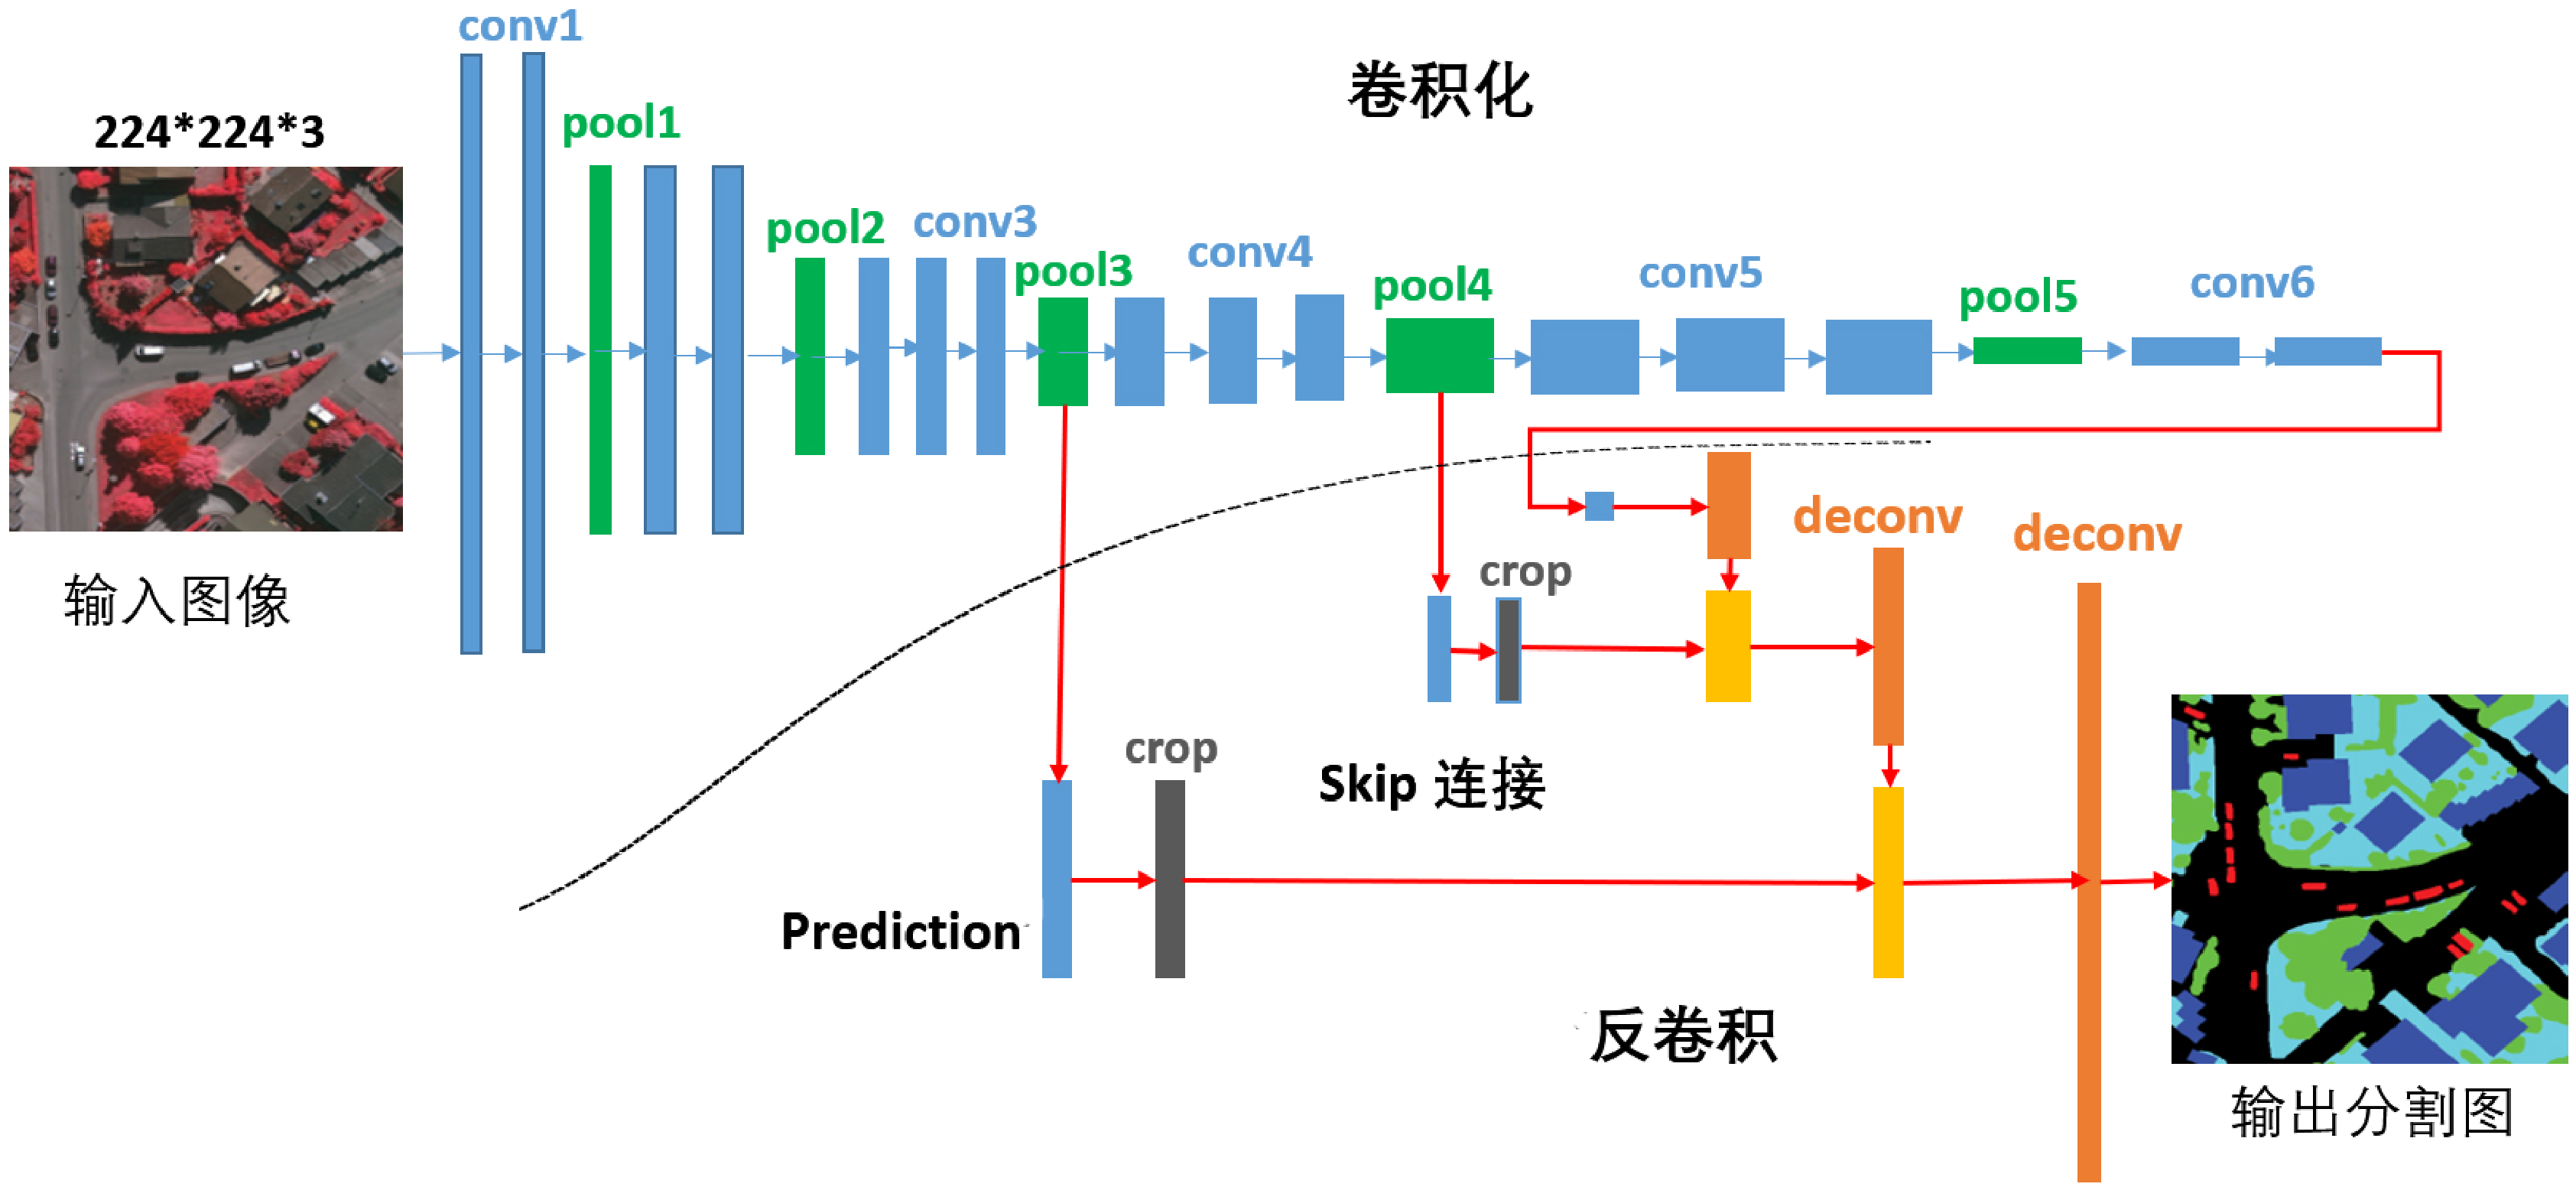
\includegraphics[width=1.0\textwidth]{figures/vgg-fcn}
  \caption{基于FCN网络的遥感影像分割示意图}\label{fig:vgg-fcn}
\end{figure}

\section{本章小结}
\label{sec:chap02-3}
balabala